% !TeX program = xelatex
% 从现有立方体平行投影视角中抽出的三维原生转换样例。
\documentclass[11pt,tikz,border=8pt]{standalone}

\usepackage{amsmath}
\usetikzlibrary{arrows.meta,perspective}

\definecolor{ink}{HTML}{26343B}
\definecolor{hidden}{HTML}{7B8A91}
\definecolor{axisx}{HTML}{C95C45}
\definecolor{axisy}{HTML}{3B8A5A}
\definecolor{axisz}{HTML}{2F6FA3}
\definecolor{facegold}{HTML}{E7B45D}
\definecolor{faceblue}{HTML}{71A9C8}
\definecolor{facegreen}{HTML}{6EAD88}

\begin{document}

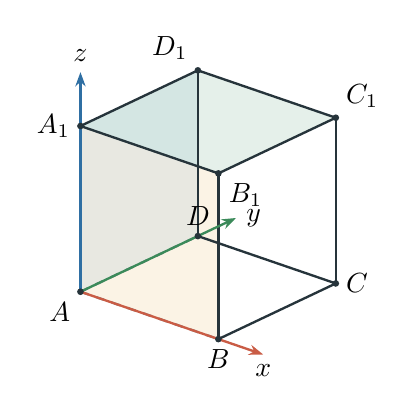
\begin{tikzpicture}[
  3d view={40.4}{23.8},
  scale=1.15,
  line width=0.85pt,
  line cap=round,
  line join=round
]
  \coordinate (A) at (0,0,0);
  \coordinate (B) at (2,0,0);
  \coordinate (C) at (2,2,0);
  \coordinate (D) at (0,2,0);
  \coordinate (A1) at (0,0,2);
  \coordinate (B1) at (2,0,2);
  \coordinate (C1) at (2,2,2);
  \coordinate (D1) at (0,2,2);

  \coordinate (X) at (2.65,0,0);
  \coordinate (Y) at (0,2.65,0);
  \coordinate (Z) at (0,0,2.65);

  \fill[facegold,fill opacity=0.16] (A)--(B)--(B1)--(A1)--cycle;
  \fill[faceblue,fill opacity=0.14] (A)--(D)--(D1)--(A1)--cycle;
  \fill[facegreen,fill opacity=0.18] (A1)--(B1)--(C1)--(D1)--cycle;

  \draw[hidden,dashed] (A)--(B);
  \draw[hidden,dashed] (A)--(D);
  \draw[hidden,dashed] (A)--(A1);

  \draw[ink] (B)--(C)--(D);
  \draw[ink] (B)--(B1);
  \draw[ink] (C)--(C1);
  \draw[ink] (D)--(D1);
  \draw[ink] (A1)--(B1)--(C1)--(D1)--cycle;

  \draw[-{Stealth[length=1.8mm,width=1.3mm]},axisx] (A)--(X);
  \draw[-{Stealth[length=1.8mm,width=1.3mm]},axisy] (A)--(Y);
  \draw[-{Stealth[length=1.8mm,width=1.3mm]},axisz] (A)--(Z);

  \fill[ink] (A) circle (1.05pt);
  \fill[ink] (B) circle (1.05pt);
  \fill[ink] (C) circle (1.05pt);
  \fill[ink] (D) circle (1.05pt);
  \fill[ink] (A1) circle (1.05pt);
  \fill[ink] (B1) circle (1.05pt);
  \fill[ink] (C1) circle (1.05pt);
  \fill[ink] (D1) circle (1.05pt);

  \node[below left] at (A) {$A$};
  \node[below] at (B) {$B$};
  \node[right] at (C) {$C$};
  \node[above] at (D) {$D$};
  \node[left] at (A1) {$A_1$};
  \node[below right] at (B1) {$B_1$};
  \node[above right] at (C1) {$C_1$};
  \node[above left] at (D1) {$D_1$};

  \node[below] at (X) {$x$};
  \node[right] at (Y) {$y$};
  \node[above] at (Z) {$z$};
\end{tikzpicture}

\end{document}
